\documentclass{beamer}
\usepackage{preamble}

\title[Théorie des groupes]
{Utilisation de modules \LaTeX}

\author{\texttt{$\backslash$usepackage\{Antoine\;de\;Lagrave\}}}

\institute[]{
    Introduction à \LaTeX{} \\
    Département de physique \\
    UDS / UQTR
}

\date[\today]

\begin{document}

    \setbeamercolor*{item}{fg=black}

    \frame{\titlepage}

    % ----------------
% MISE EN CONTEXTE
% ----------------

\begin{frame}
    \frametitle{Mise en contexte - Utilité des modules}
    Les modules (\textit{packages}) permettent d'accomplir
    des tâches et modifications non-triviales. Grâce à elles ont
    \vspace{0.3cm}
    \begin{itemize}
        \pause
        \item[$\diamond$] Sauve parfois beaucoup de temps
        \item[$\diamond$] Automatise des tâches complexes
        \item[$\diamond$] Rend l'usage de \LaTeX\;plus agréable et professionnel
    \end{itemize}
    \vfill
    \pause
    \begin{noteblock}{Note: Temps de compilation}
        Les modules sont parfois très lourdes\dots\;S'il est possible de l'éviter
        facilement, n'importez pas de nouveau(x) modules(s)!
    \end{noteblock}
\end{frame}

\begin{frame}[fragile]
    \frametitle{Mise en contexte - Utilité des modules}
    Pour utiliser un module, on l'importe dans le préambule \textcolor{hard_green}{avant la création du
    document} via la commande
    \vfill
    \begin{lstlisting}[xleftmargin=-10mm]
        \usepackage[option1, option2, ...]{package},
    \end{lstlisting}
    \vfill
    où ici les options sont facultatives.
\end{frame}


    \begin{frame}
        \frametitle{Table des matières}
        \tableofcontents
    \end{frame}

    % -----------------------------
% PERSONNALISATION DE DOCUMENTS
% -----------------------------

% Defining TOC's sections before content
\section{Personnalisation de documents}

\subsection{Mise en page}

\subsection{En-têtes, pieds de page et sections}

\begin{frame}
    \vfill
    \begin{center}
        \large
        Personnalisation de documents
    \end{center}
    \vfill
\end{frame}

\begin{frame}
    \frametitle{Personnalisation de documents - Mise en page}
    Module \textcolor{vibrant_green}{\textit{geometry}}\footnotemark permet de gérer les dimensions des pages.
    \begin{figure}
        \centering
            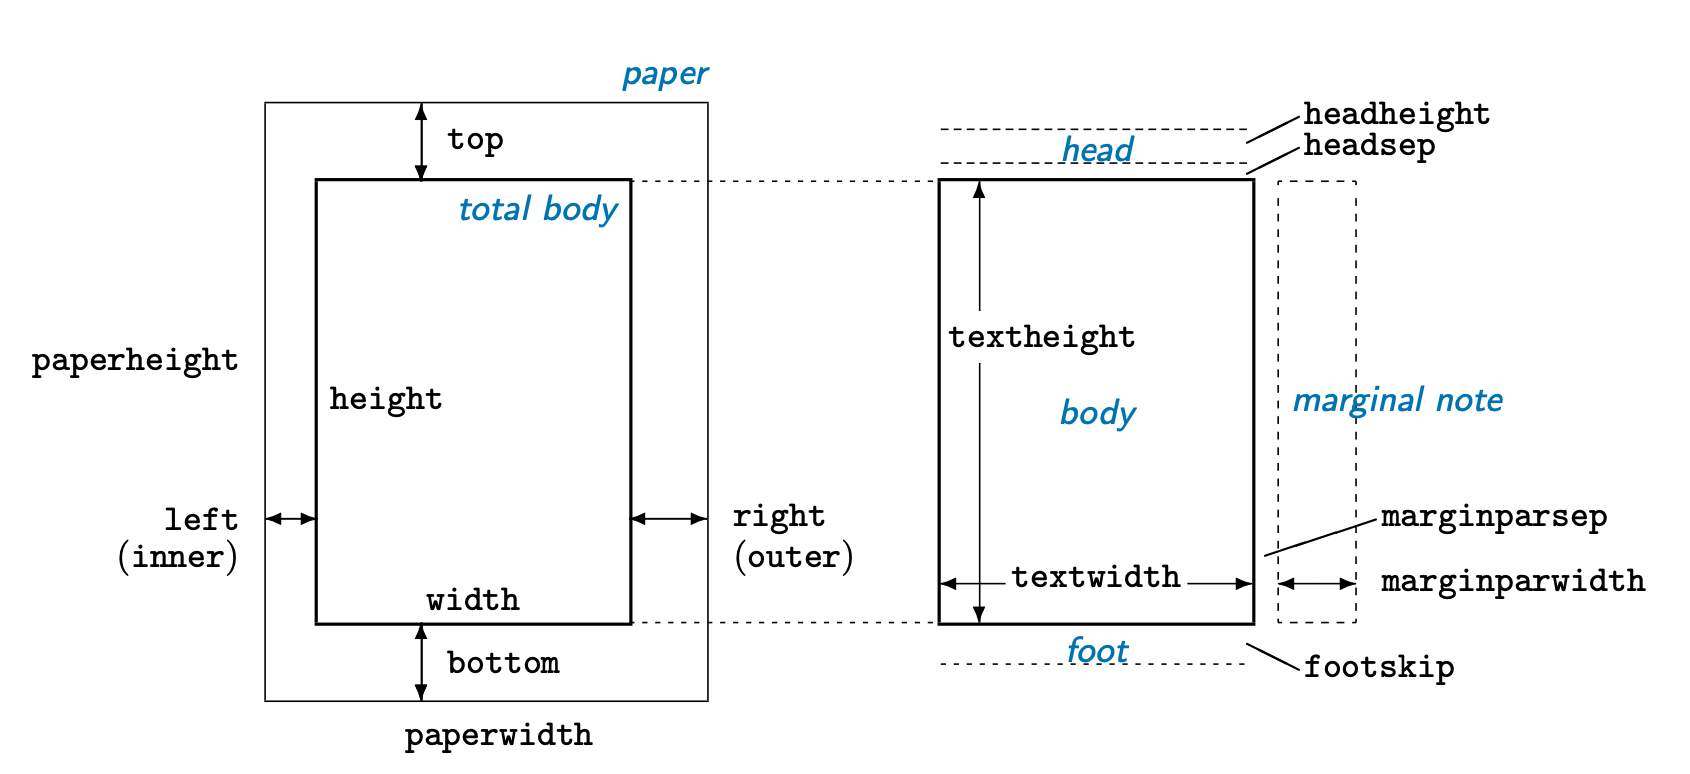
\includegraphics[scale=0.35]{./figures/geometry.png}
            \label{fig: geometry}
    \end{figure}
    \footnotetext{geometry – Flexible and complete interface to document dimensions. \href{https://ctan.org/pkg/geometry}{\textcolor{vibrant_green}{https://ctan.org/pkg/geometry}}.}
\end{frame}

\begin{frame}[fragile]
    \frametitle{Personnalisation de documents - Mise en page}
    Les commandes suivantes pour modifier les dimensions sont équivalentes
    \vfill
    \begin{lstlisting}[xleftmargin=-10mm]
        \usepackage[height=10in, a5paper]{geometry}
    \end{lstlisting}
    \vfill
    \centering
    où
    \vfill
    \begin{lstlisting}[xleftmargin=-10mm]
        \usepackage{geometry}
        \geometry{height=10in, a5paper}
    \end{lstlisting}
\end{frame}

\begin{frame}[fragile]
    \frametitle{Personnalisation de documents - En-têtes, pieds de page et sections}
    Avec \textcolor{vibrant_green}{\textit{fancyhdr}}\footnotemark, on personnalise les en-têtes et pieds de page grâce à l'utilisation d'un nouveau style de page
    \vfill
    \begin{lstlisting}[xleftmargin=1cm]
        \usepackage{fancyhdr}
        \pagestyle{fancy}
    \end{lstlisting}
    \footnotetext{fancyhdr – Extensive control of page headers and footers in \LaTeX. \href{https://ctan.org/pkg/fancyhdr}{\textcolor{vibrant_green}{https://ctan.org/pkg/fancyhdr}}.}
\end{frame}

\begin{frame}[fragile]
    \frametitle{Personnalisation de documents - En-têtes, pieds de page et sections}
    Avec \textcolor{vibrant_green}{\textit{fancyhdr}}\footnotemark, on personnalise les en-têtes et pieds de page grâce à l'utilisation d'un nouveau style de page
    \vfill
    \begin{figure}
        \centering
            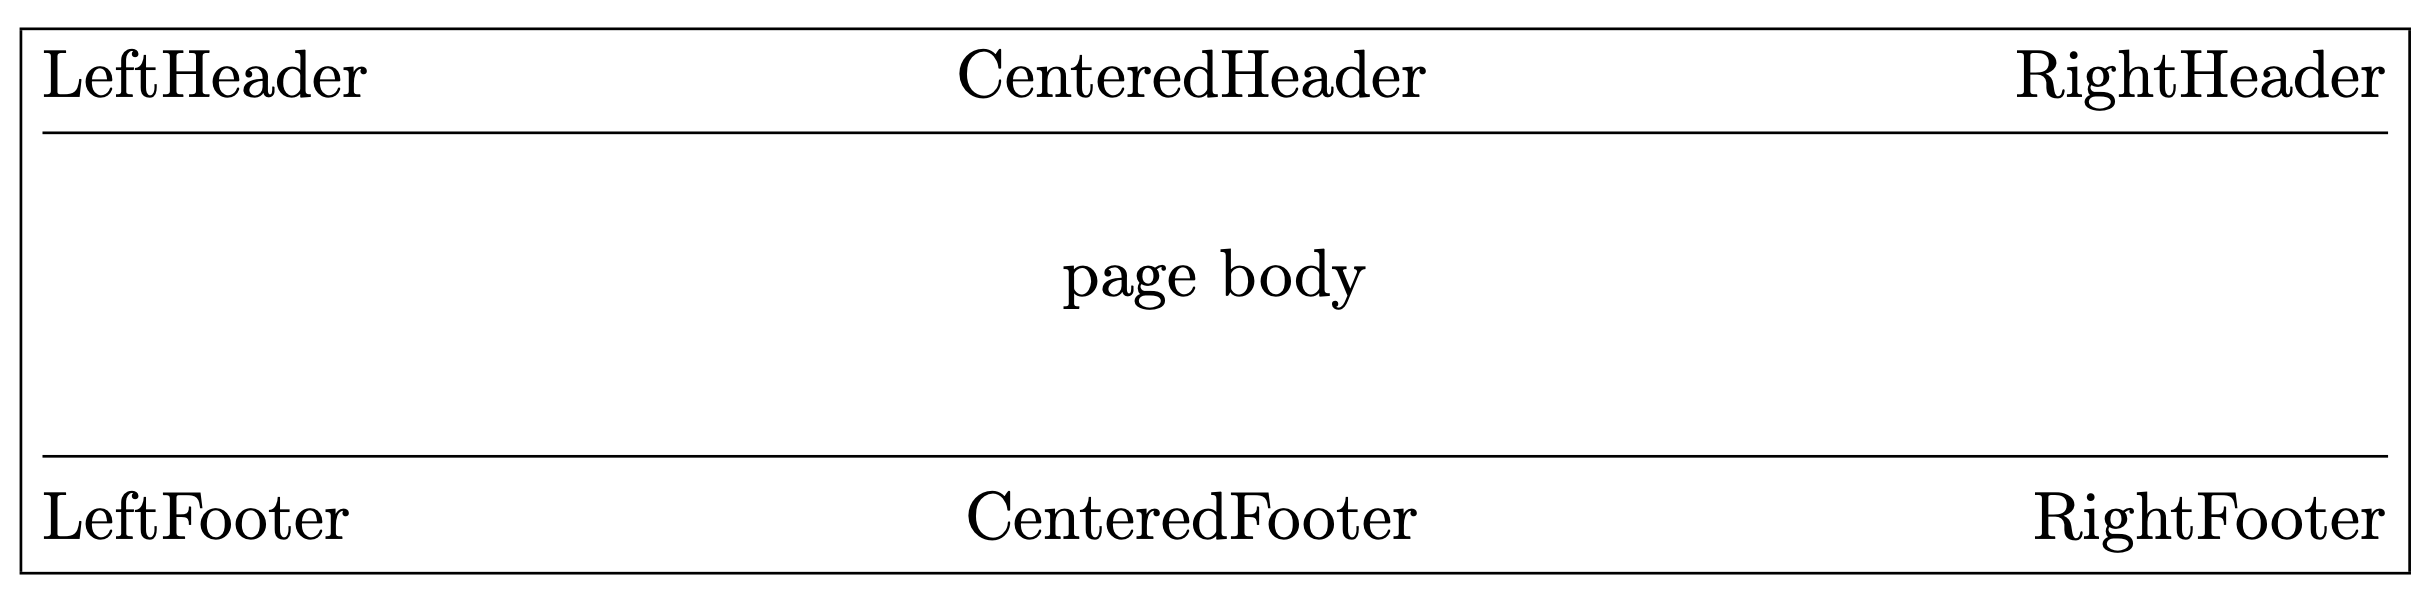
\includegraphics[scale=0.25]{./figures/fancyhdr.png}
            \label{fig: fancyhdr}
    \end{figure}
    \footnotetext{fancyhdr – Extensive control of page headers and footers in \LaTeX. \href{https://ctan.org/pkg/fancyhdr}{\textcolor{vibrant_green}{https://ctan.org/pkg/fancyhdr}}.}
\end{frame}

\begin{frame}[fragile]
    \frametitle{Personnalisation de documents - En-têtes, pieds de page et sections}
    Prenons par exemple le code suivant
    \vfill
    \begin{lstlisting}[xleftmargin=-1.75cm]
        \fancyhead[L,C]{}
        \fancyhead[R]{\textbf{The performance of new graduates}}
        \fancyfoot[L]{From: K. Grant}
        \fancyfoot[C]{To: Dean A. Smith}
        \fancyfoot[R]{\thepage}
        \renewcommand{\headrulewidth}{0.4pt}
        \renewcommand{\footrulewidth}{2pt}
    \end{lstlisting}
    \vfill
\end{frame}

\begin{frame}[fragile]
    \frametitle{Personnalisation de documents - En-têtes, pieds de page et sections}
    Qui permet d'obtenir
    \vfill
    \begin{figure}
        \centering
            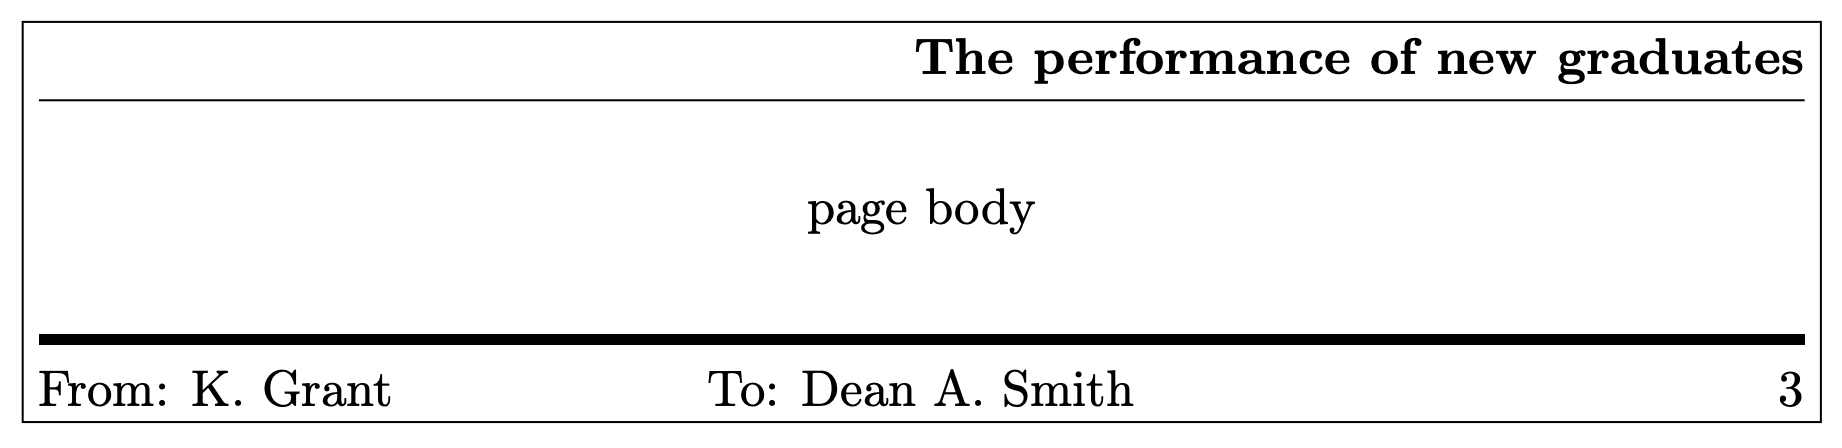
\includegraphics[scale=0.3]{./figures/fancyhdr_2.png}
            \label{fig: fancyhdr_2}
    \end{figure}
    \vfill
\end{frame}

\begin{frame}
    \frametitle{Personnalisation de documents - En-têtes, pieds de page et sections}
    Le module \textcolor{vibrant_green}{\textit{titlesec}}\footnotemark permet de choisir le format des titres de sections, sous-sections et etc.
    \begin{columns}
        \column{0.5\linewidth}
        \begin{figure}
           \centering
            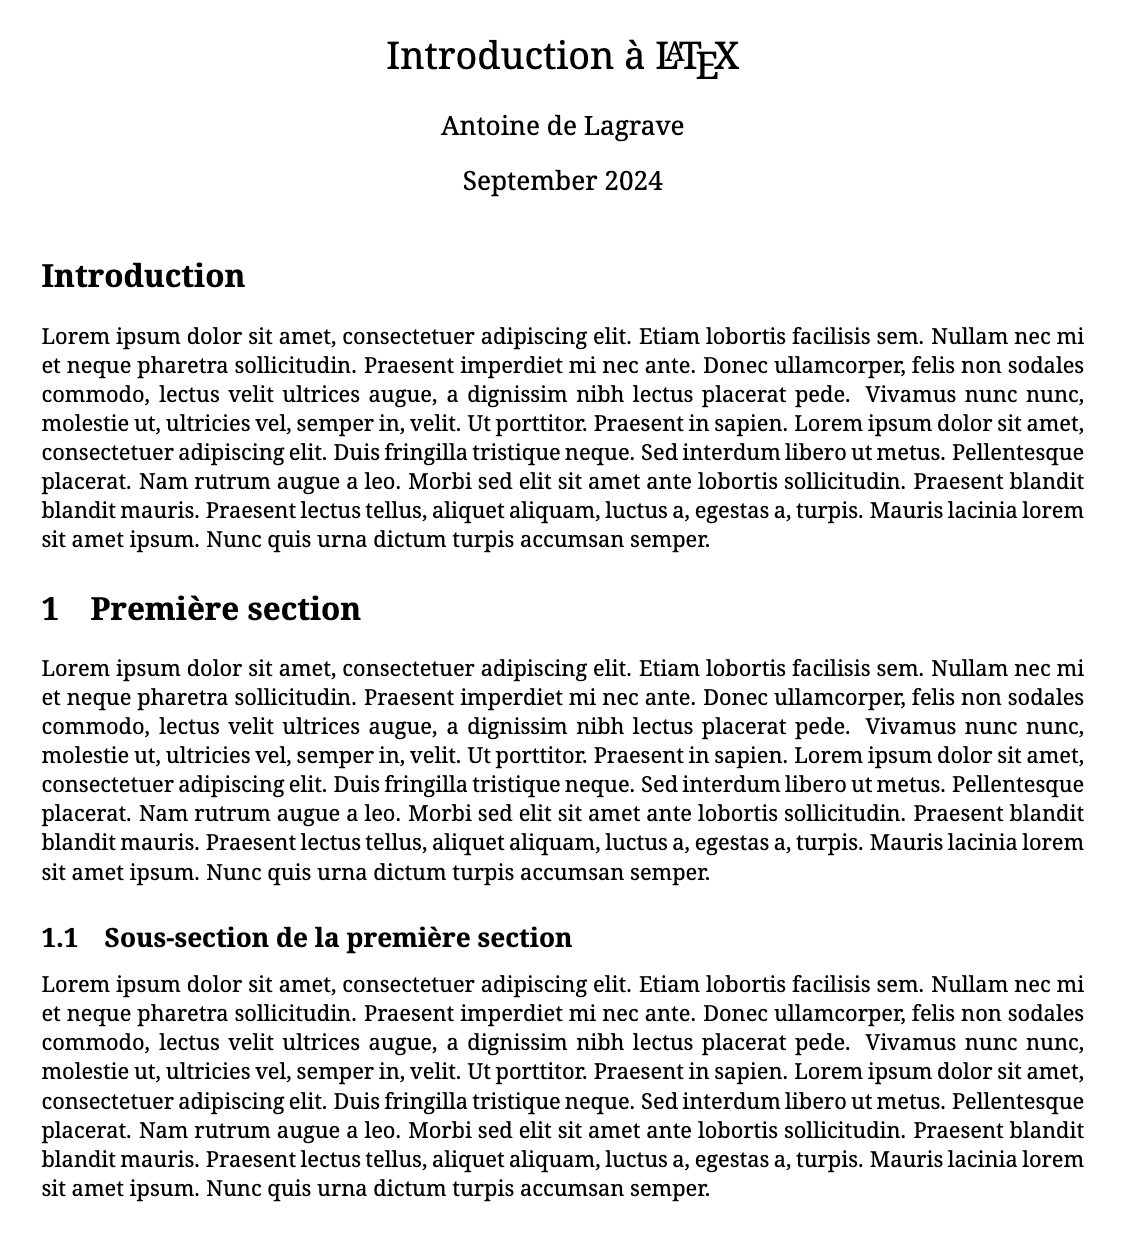
\includegraphics[scale=0.2]{./figures/titlesec.png}
            \label{fig: titlesec}
        \end{figure}
        \column{0.5\linewidth}
        \begin{figure}
           \centering
            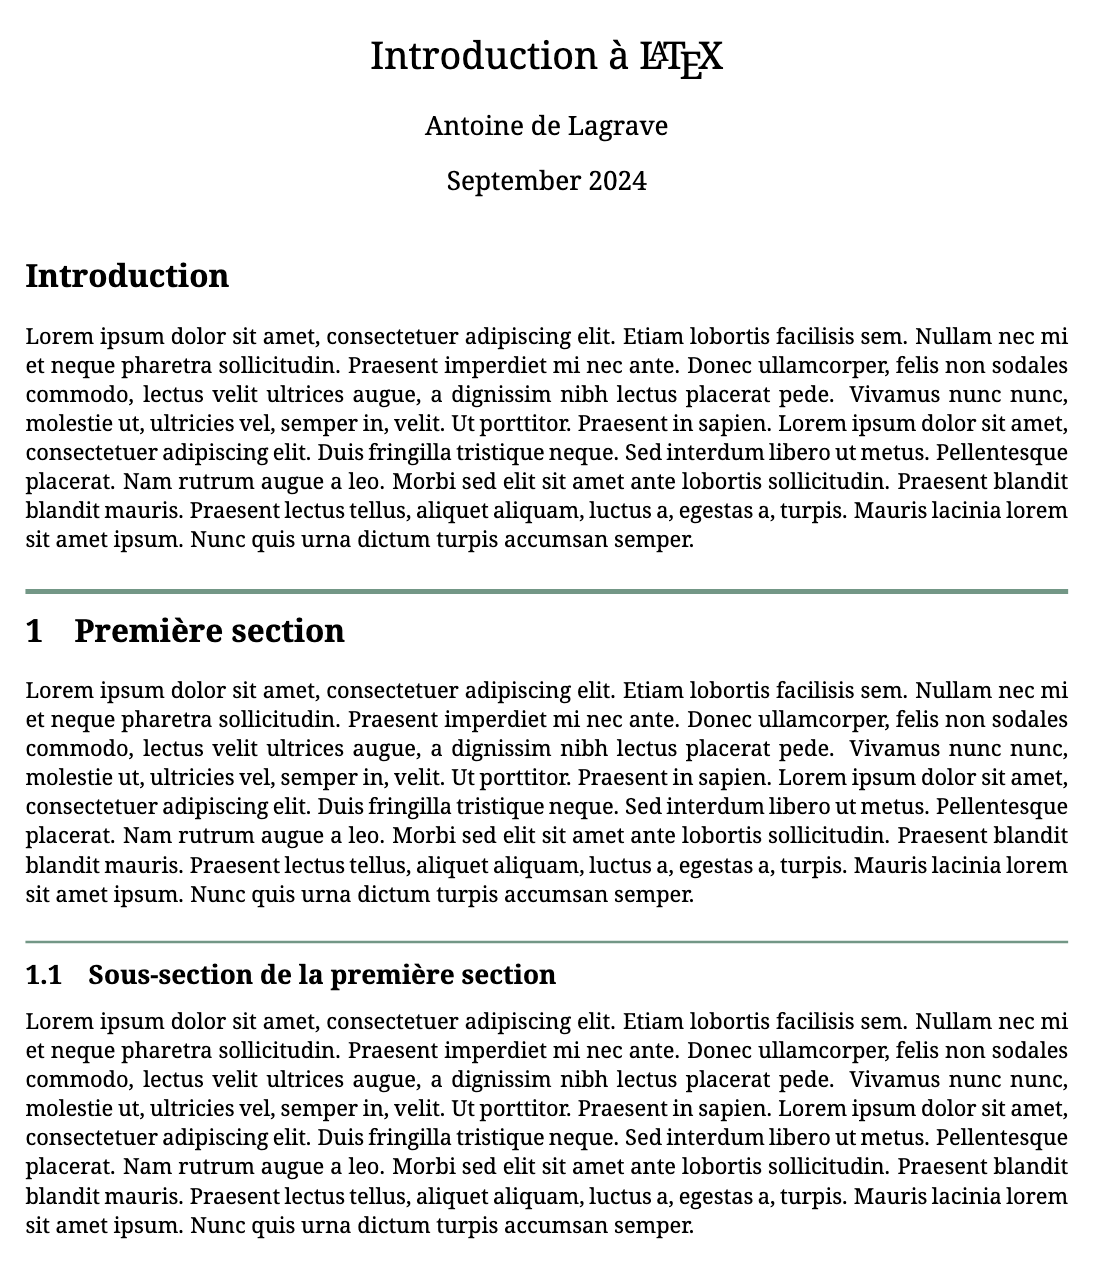
\includegraphics[scale=0.2]{./figures/titlesec_2.png}
            \label{fig: titlesec_2}
        \end{figure}
    \end{columns}
    \footnotetext{titlesec – Select alternative section titles. \href{https://ctan.org/pkg/titlesec}{\textcolor{vibrant_green}{https://ctan.org/pkg/titlesec}}.}
\end{frame}


    % -------------------------
% Physique et Mathématiques
% -------------------------

% Defining TOC's sections before content
\section{Physique et Mathématiques}

\subsection{Module \textit{physics}}

\subsection{Mathématiques avancés}

\begin{frame}
    \vfill
    \begin{center}
        \large
        Physique et Mathématiques
    \end{center}
    \vfill
\end{frame}

\begin{frame}
    \frametitle{Physique et Mathématiques - Module \textit{physics}}
    Le module \textcolor{hard_green}{\textit{physics}}\footnotemark est de loin un des outils les plus utiles via
    \pause
    \vspace{0.3cm}
    \begin{itemize}
        \item[$\diamond$] Gestion de parenthèses
        \item[$\diamond$] Notation vectorielle
        \item[$\diamond$] Opérateurs mathématiques ($\sin, \det, \Trace,\dots$)
        \item[$\diamond$] Notation différentielle (dérivées et dérivées partielles)
        \item[$\diamond$] Raccourcis pour les matrices
        \item[$\diamond$] Notation de Dirac
    \end{itemize}
    \footnotetext{physics – Macros supporting the Mathematics of Physics. \href{https://ctan.org/pkg/physics}{\textcolor{hard_green}{https://ctan.org/pkg/physics}}.}
\end{frame}

\begin{frame}[fragile]
    \frametitle{Physique et Mathématiques - Module \textit{physics}}
    \begin{columns}
        \column{0.55\linewidth}
        \begin{lstlisting}[xleftmargin=-2cm]
            \qty(\frac{1}{2})^n


            \norm{\vb{v}}


            \pdv[3]{f}{x}


            \smqty{\imat{3}}
        \end{lstlisting}
        \column{0.45\linewidth}
        \vspace{-0.3cm}
        \begin{align*}
            &\qty(\frac{1}{2})^n\qq{vs}(\frac{1}{2})^n \\\\
            &\norm{\vb{v}} \\\\
            &\pdv[3]{f}{x} \\\\
            &\smqty(\imat{3})
        \end{align*}
    \end{columns}
\end{frame}

\begin{frame}
  \frametitle{Physique et Mathématiques - Mathématiques avancés}
  L'essentiel en termes de notation mathématique peut être résumé par les modules
  \vspace{0.3cm}
  \pause
    \begin{itemize}
        \item[$\diamond$] \textcolor{hard_green}{\textit{amsmath}}\footnotemark (environnements mathématiques)
        \footnotetext{amsmath – AMS mathematical facilities for \LaTeX. \href{https://ctan.org/pkg/amsmath}{\textcolor{hard_green}{https://ctan.org/pkg/amsmath}}.}
        \item[$\diamond$] \textcolor{hard_green}{\textit{amsfonts}}\footnotemark (styles calligraphiques: $\mathcal{A}, \mathcal{B}, \mathcal{C}$)
        \footnotetext{amsfonts – TeX fonts from the American Mathematical Society. \href{https://ctan.org/pkg/amsfonts}{\textcolor{hard_green}{https://ctan.org/pkg/amsfonts}}.}
        \item[$\diamond$] \textcolor{hard_green}{\textit{amsthm}}\footnotemark(théorèmes, preuves, définitions)
        \footnotetext{amsthm – Typesetting theorems (AMS style). \href{https://ctan.org/pkg/amsthm}{\textcolor{hard_green}{https://ctan.org/pkg/amsthm}}.}
        \item[$\diamond$] \textcolor{hard_green}{\textit{dsfont}}\footnotemark (lettres doubles pour les ensembles: $\mathds{R}, \mathds{N}, \mathds{Z}$)
    \end{itemize}
    \footnotetext{doublestroke – Typeset mathematical double stroke symbols. \href{https://ctan.org/pkg/doublestroke}{\textcolor{hard_green}{https://ctan.org/pkg/doublestroke}}.}
\end{frame}

\begin{frame}
  \frametitle{Physique et Mathématiques - Mathématiques avancés}
  Les environnements mathématiques permettent notamment d'aligner des équations lors d'un développement
    \begin{align*}
        \mathrm{H}\ket{\ell, S, J, M_J} &= \frac{\vb{L}^2}{2I}\ket{\ell, S, J, M_J} + \frac{\alpha}{2}\qty[\vb{J}^2 - \vb{L}^2 - \vb{S}^2]\ket{\ell, S, J, M_J} \\\\
        &= \frac{\hbar^2}{2}\qty[\frac{\ell(\ell + 1)}{I} + \alpha\qty(J(J + 1) - \ell(\ell + 1) - \frac{3}{4})]\ket{\ell, S, J, M_J} \\\\
        &= \frac{\hbar^2}{2}\qty[\ell(\ell + 1)\qty(\frac{1}{I} - \alpha) + \alpha J(J + 1) - \frac{3\alpha}{4}]\ket{\ell, S, J, M_J}.
    \end{align*}
\end{frame}


    % --------------------------------------
% BIBLIOGRAPHIE, CITATIONS ET RÉFÉRENCES
% --------------------------------------

% Defining TOC's sections before content
\section{Bibliographie, citations et références}

\begin{frame}
    \vfill
    \begin{center}
        \large
        Bibliographie, citations et références
    \end{center}
    \vfill
\end{frame}

\begin{frame}
    \frametitle{Bibliographie, citations et références}
    La gestion de la bibliographie et des citations peut se faire avec \textcolor{vibrant_green}{\textit{biblatex}}\footnotemark. Il y a 4 étapes essentielles
    \vspace{0.3cm}
    \begin{itemize}
    \pause
        \item[$1.$] Importer le module et personnaliser le style
            \pause
        \item[$2.$] Créer un fichier .bib et l'ajouter comme référence
            \pause
        \item[$3.$] Citer grâce à la commande \texttt{cite\{\dots\}}
            \pause
        \item[$4.$] Insérer la bibliographie
    \end{itemize}
    \footnotetext{Bib\LaTeX – Sophisticated Bibliographies in \LaTeX. \href{https://ctan.org/pkg/biblatex}{\textcolor{vibrant_green}{https://ctan.org/pkg/biblatex}}.}
\end{frame}

\begin{frame}[fragile]
    \frametitle{Bibliographie, citations et références}
    \underline{Étape 1}:
    \begin{lstlisting}[xleftmargin=-1.5cm, basicstyle=\small]
        \usepackage[backend=biber,style=phys]{biblatex}
    \end{lstlisting}
    \vfill
    \pause
    \underline{Étape 2}:
    \begin{lstlisting}[xleftmargin=-1.5cm, basicstyle=\small]
        \addbibresource{references.bib}
    \end{lstlisting}
    \begin{columns}
        \column{0.5\linewidth}
        \begin{lstlisting}[xleftmargin=-1cm, basicstyle=\footnotesize]
            @article{Einstein1905,
              author  = {Albert Einstein},
              title   = {Some title},
              journal = {Annalen der Physik},
              volume  = {322},
              number  = {10},
              pages   = {891--921},
              year    = {1905},
              doi     = {10.1002/andp.19053221004}}
        \end{lstlisting}
        \column{0.5\linewidth}
        \begin{lstlisting}[xleftmargin=-1cm, basicstyle=\footnotesize]
            @misc{Doe2021,
              author    = {John Doe and Jane Smith},
              title     = {Some title},
              note      = {arXiv:2103.12345},
              year      = {2021},
              eprint    = {2103.12345},
              archivePrefix = {arXiv},
              primaryClass  = {quant-ph}}
        \end{lstlisting}
    \end{columns}
\end{frame}

\begin{frame}[fragile]
    \frametitle{Bibliographie, citations et références}
    \underline{Étapes 3 et 4}:
    \vfill
    \begin{lstlisting}[xleftmargin=-1cm, basicstyle=\small]
       \begin{document}

        According to \textcite{Einstein1905} ...

        \printbibliography

        \end{document}
    \end{lstlisting}
\end{frame}

\begin{frame}[fragile]
    \frametitle{Bibliographie, citations et références}
    \underline{Résultat pour un document vide}:
    \vfill
    \begin{figure}
        \centering
        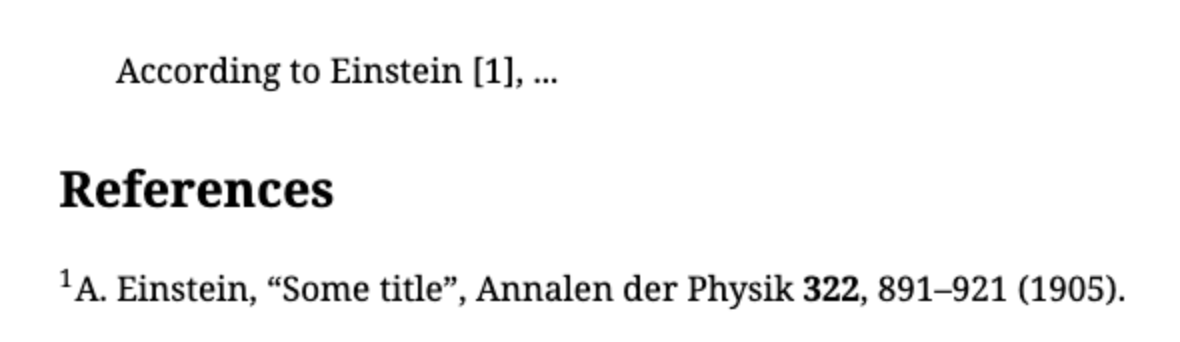
\includegraphics[width=0.65\linewidth]{./figures/biblatex.png}
        \label{fig: biblatex}
    \end{figure}
    \vfill\pause
    \begin{mybrownbox}
        \textbf{Note}~: Il est aussi possible de référencer des équations, tableaux et figures avec le module \textcolor{vibrant_green}{\textit{cleveref}}\footnotemark via la commande \texttt{cref\{...\}}.
    \end{mybrownbox}
    \footnotetext{cleveref – Intelligent cross-referencing. \href{https://ctan.org/pkg/cleveref}{\textcolor{vibrant_green}{https://ctan.org/pkg/cleveref}}.}
\end{frame}


    % ---------------------
% GRAPHIQUES ET FIGURES
% ---------------------

% Defining TOC's sections before content
\section{Graphiques et figures}

\begin{frame}
    \vfill
    \begin{center}
        \large
        Graphiques et figures
    \end{center}
    \vfill
\end{frame}

\begin{frame}
    \frametitle{Graphiques et figures}
    Un module pratique pour la mise en page de figures est \textcolor{hard_green}{\textit{subfloat}}\footnotemark. Celle-ci permet de mettre plusieurs sous-figures dans un même environnement.
    \vfill
    \begin{figure}
        \centering
        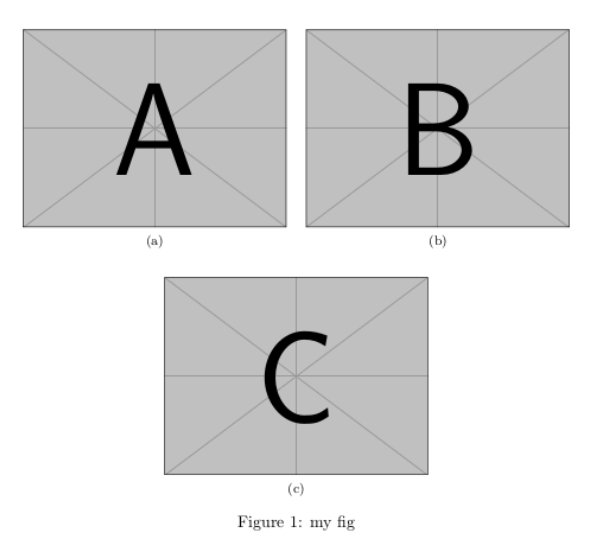
\includegraphics[width=0.4\linewidth]{./figures/subfloat.png}
        \label{fig: subfloat}
    \end{figure}
    \footnotetext{subfloat – Sub-numbering for figures and tables. \href{https://ctan.org/pkg/subfloat}{\textcolor{hard_green}{https://ctan.org/pkg/subfloat}}.}
\end{frame}

\begin{frame}
    \frametitle{Graphiques et figures}
    Un autre module utile pour la mise en page de figures est \textcolor{hard_green}{\textit{wrapfig}}\footnotemark. Celle-ci permet d'insérer une figure à l'intérieur d'une zone de texte.
    \vfill
    \begin{figure}
        \centering
        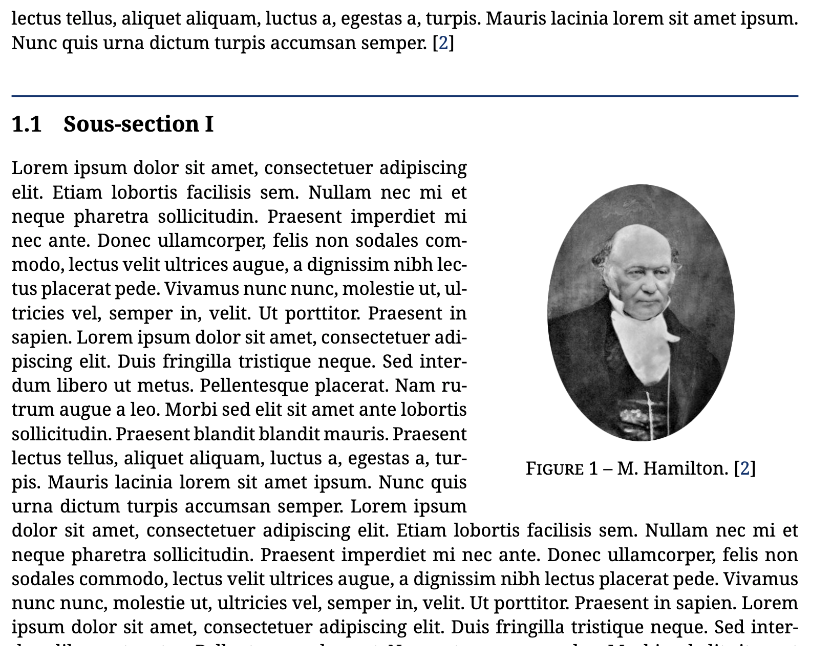
\includegraphics[width=0.45\linewidth]{./figures/wrapfig.png}
        \label{fig: wrapfig}
    \end{figure}
    \footnotetext{wrapfig – Produces figures which text can flow around. \href{https://ctan.org/pkg/wrapfig}{\textcolor{hard_green}{https://ctan.org/pkg/wrapfig}}.}
\end{frame}

\begin{frame}
    \frametitle{Graphiques et figures}
    Il existe même un module qui permet de créer ses propres figures \textit{vectorisées} nommée \textcolor{hard_green}{\textit{TikZ}}\footnotemark
    \vfill
    \pause
    \begin{columns}
        \column{0.33\linewidth}
        \begin{figure}
            \centering
            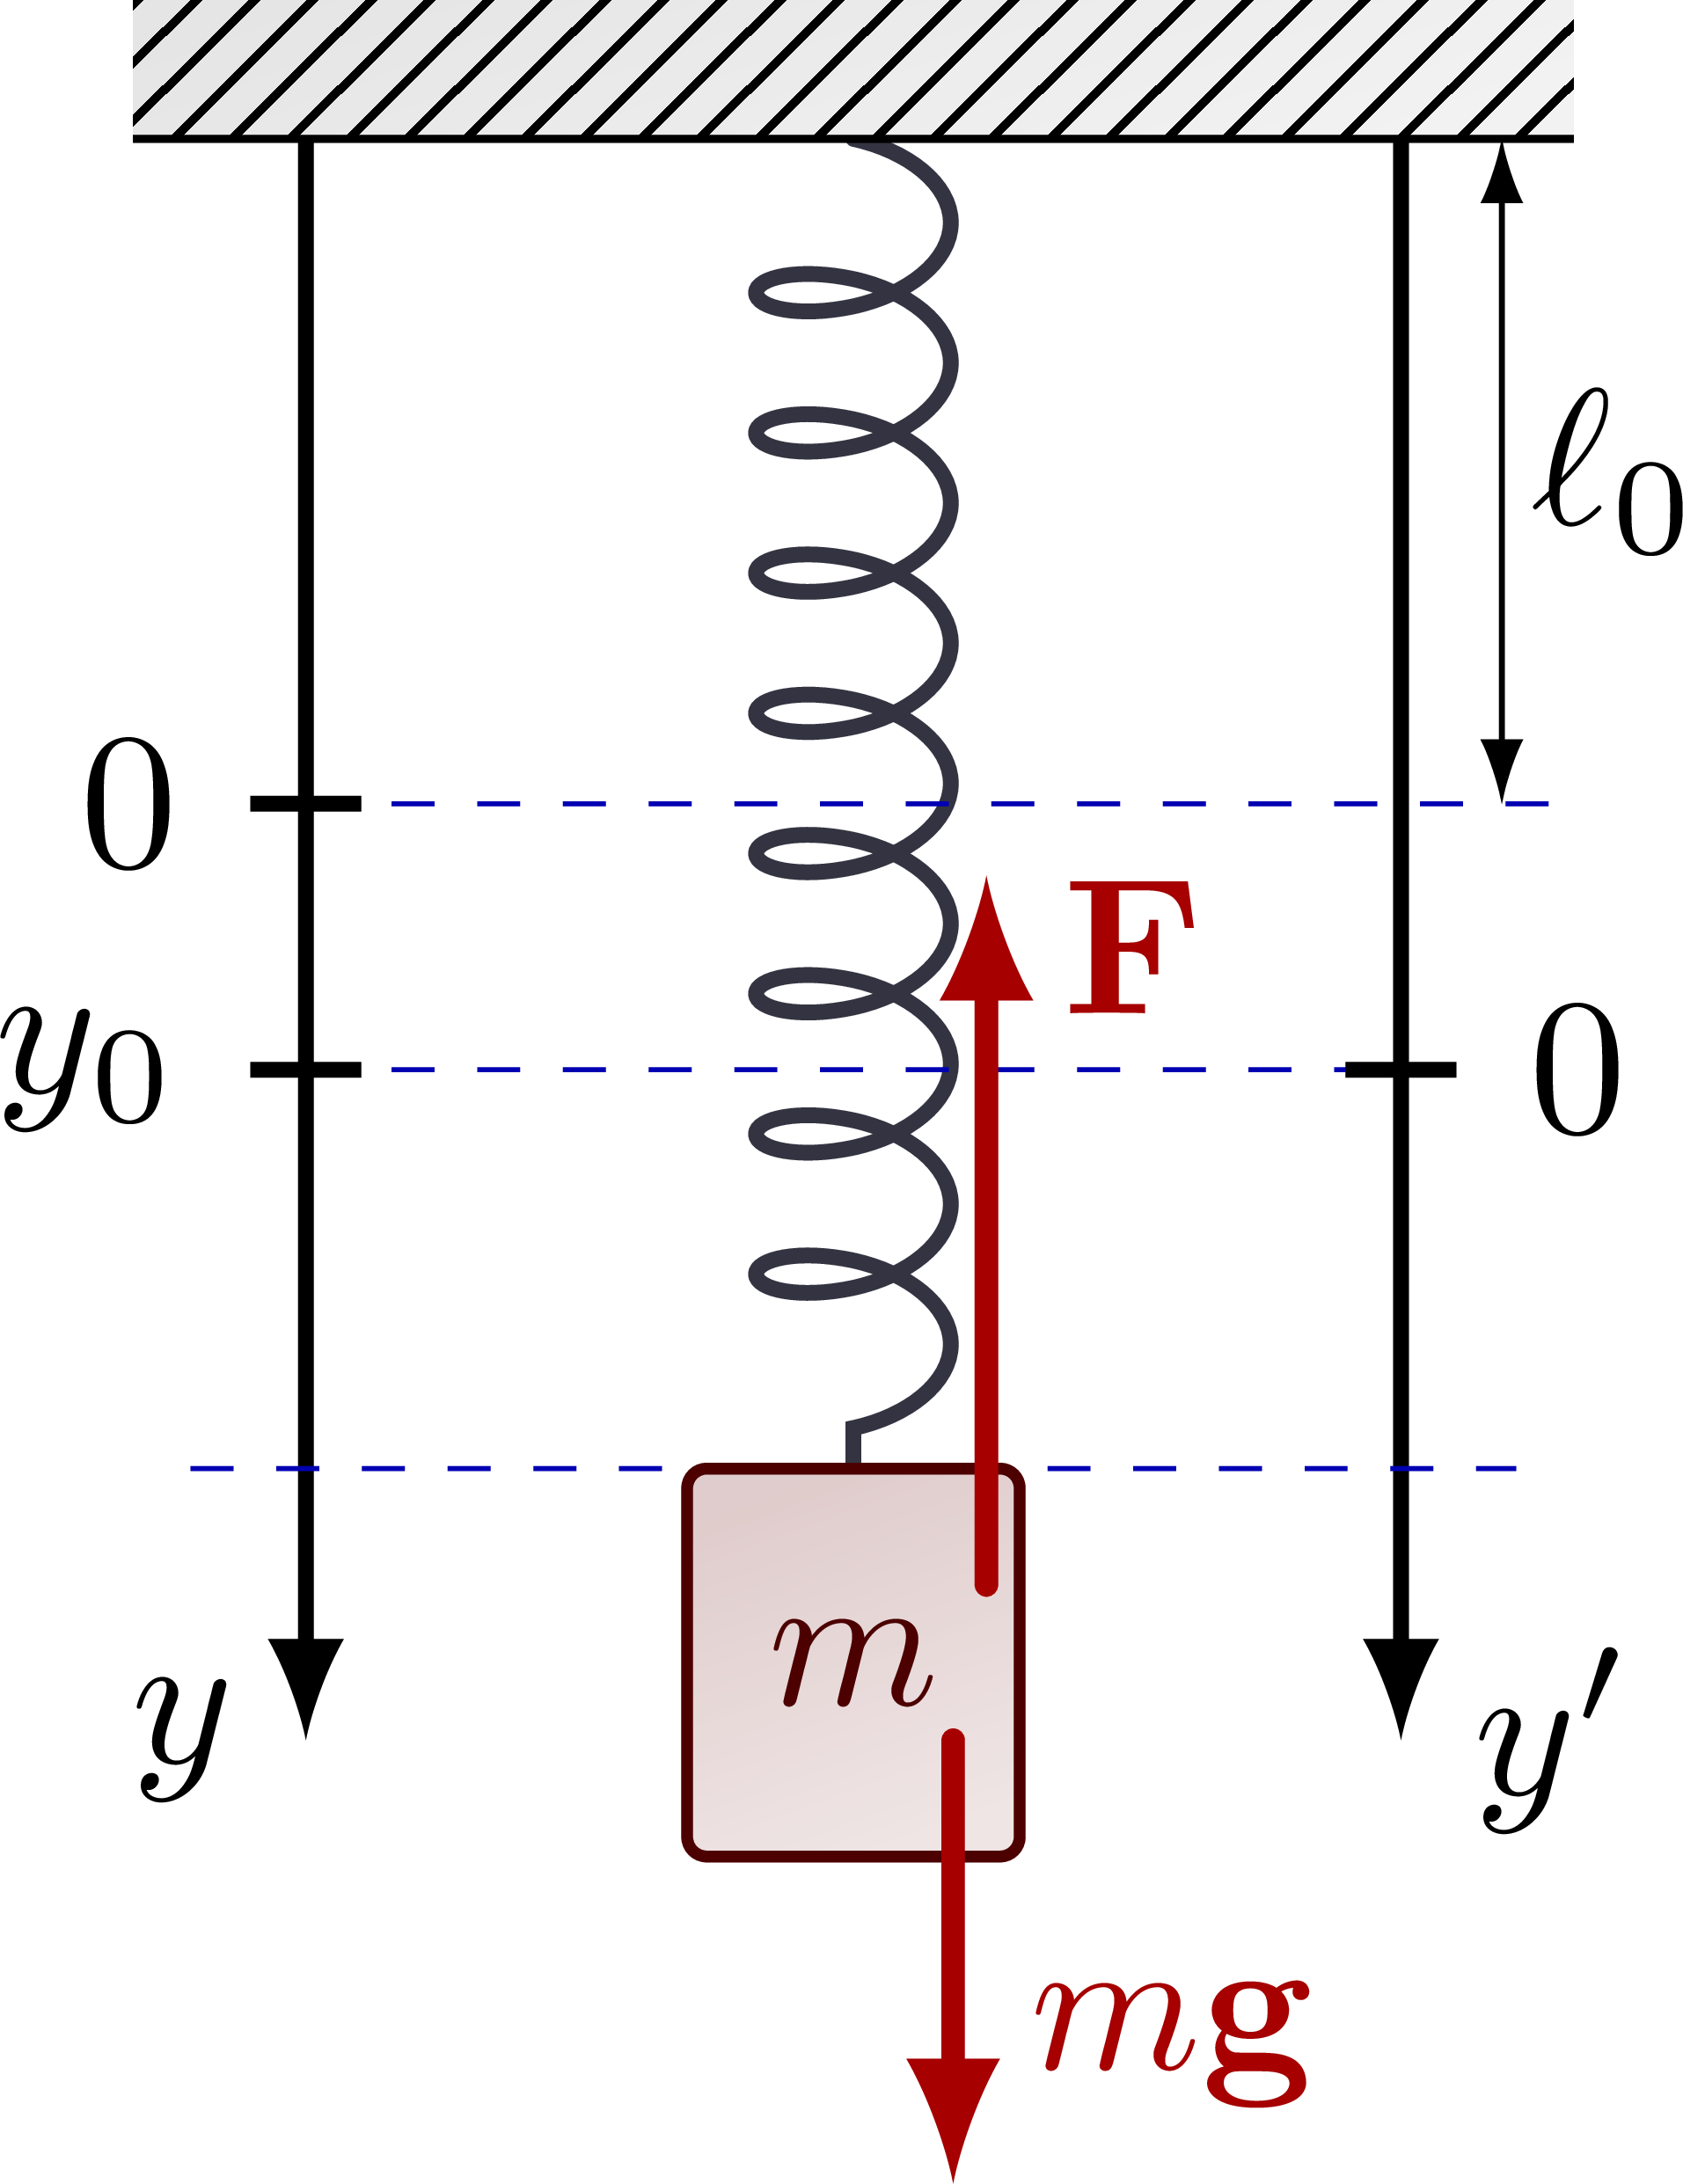
\includegraphics[width=0.55\linewidth]{./figures/tikz.png}
            \label{fig: tikz}
        \end{figure}
        \column{0.33\linewidth}
        \pause
        \begin{figure}
            \centering
            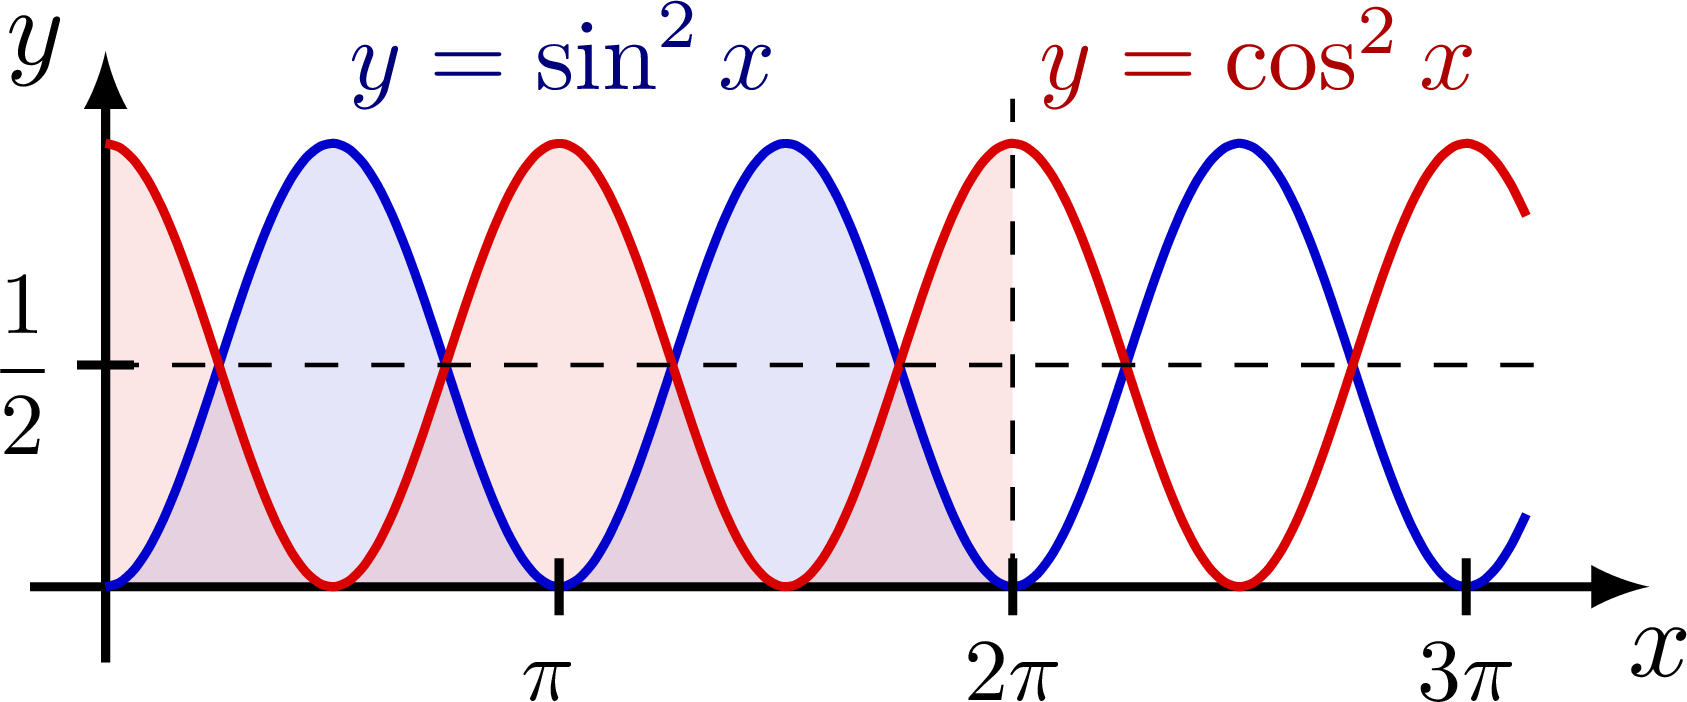
\includegraphics[width=0.9\linewidth]{./figures/tikz_2.png}
            \label{fig: tikz_2}
        \end{figure}
        \column{0.33\linewidth}
        \pause
        \begin{figure}
            \centering
            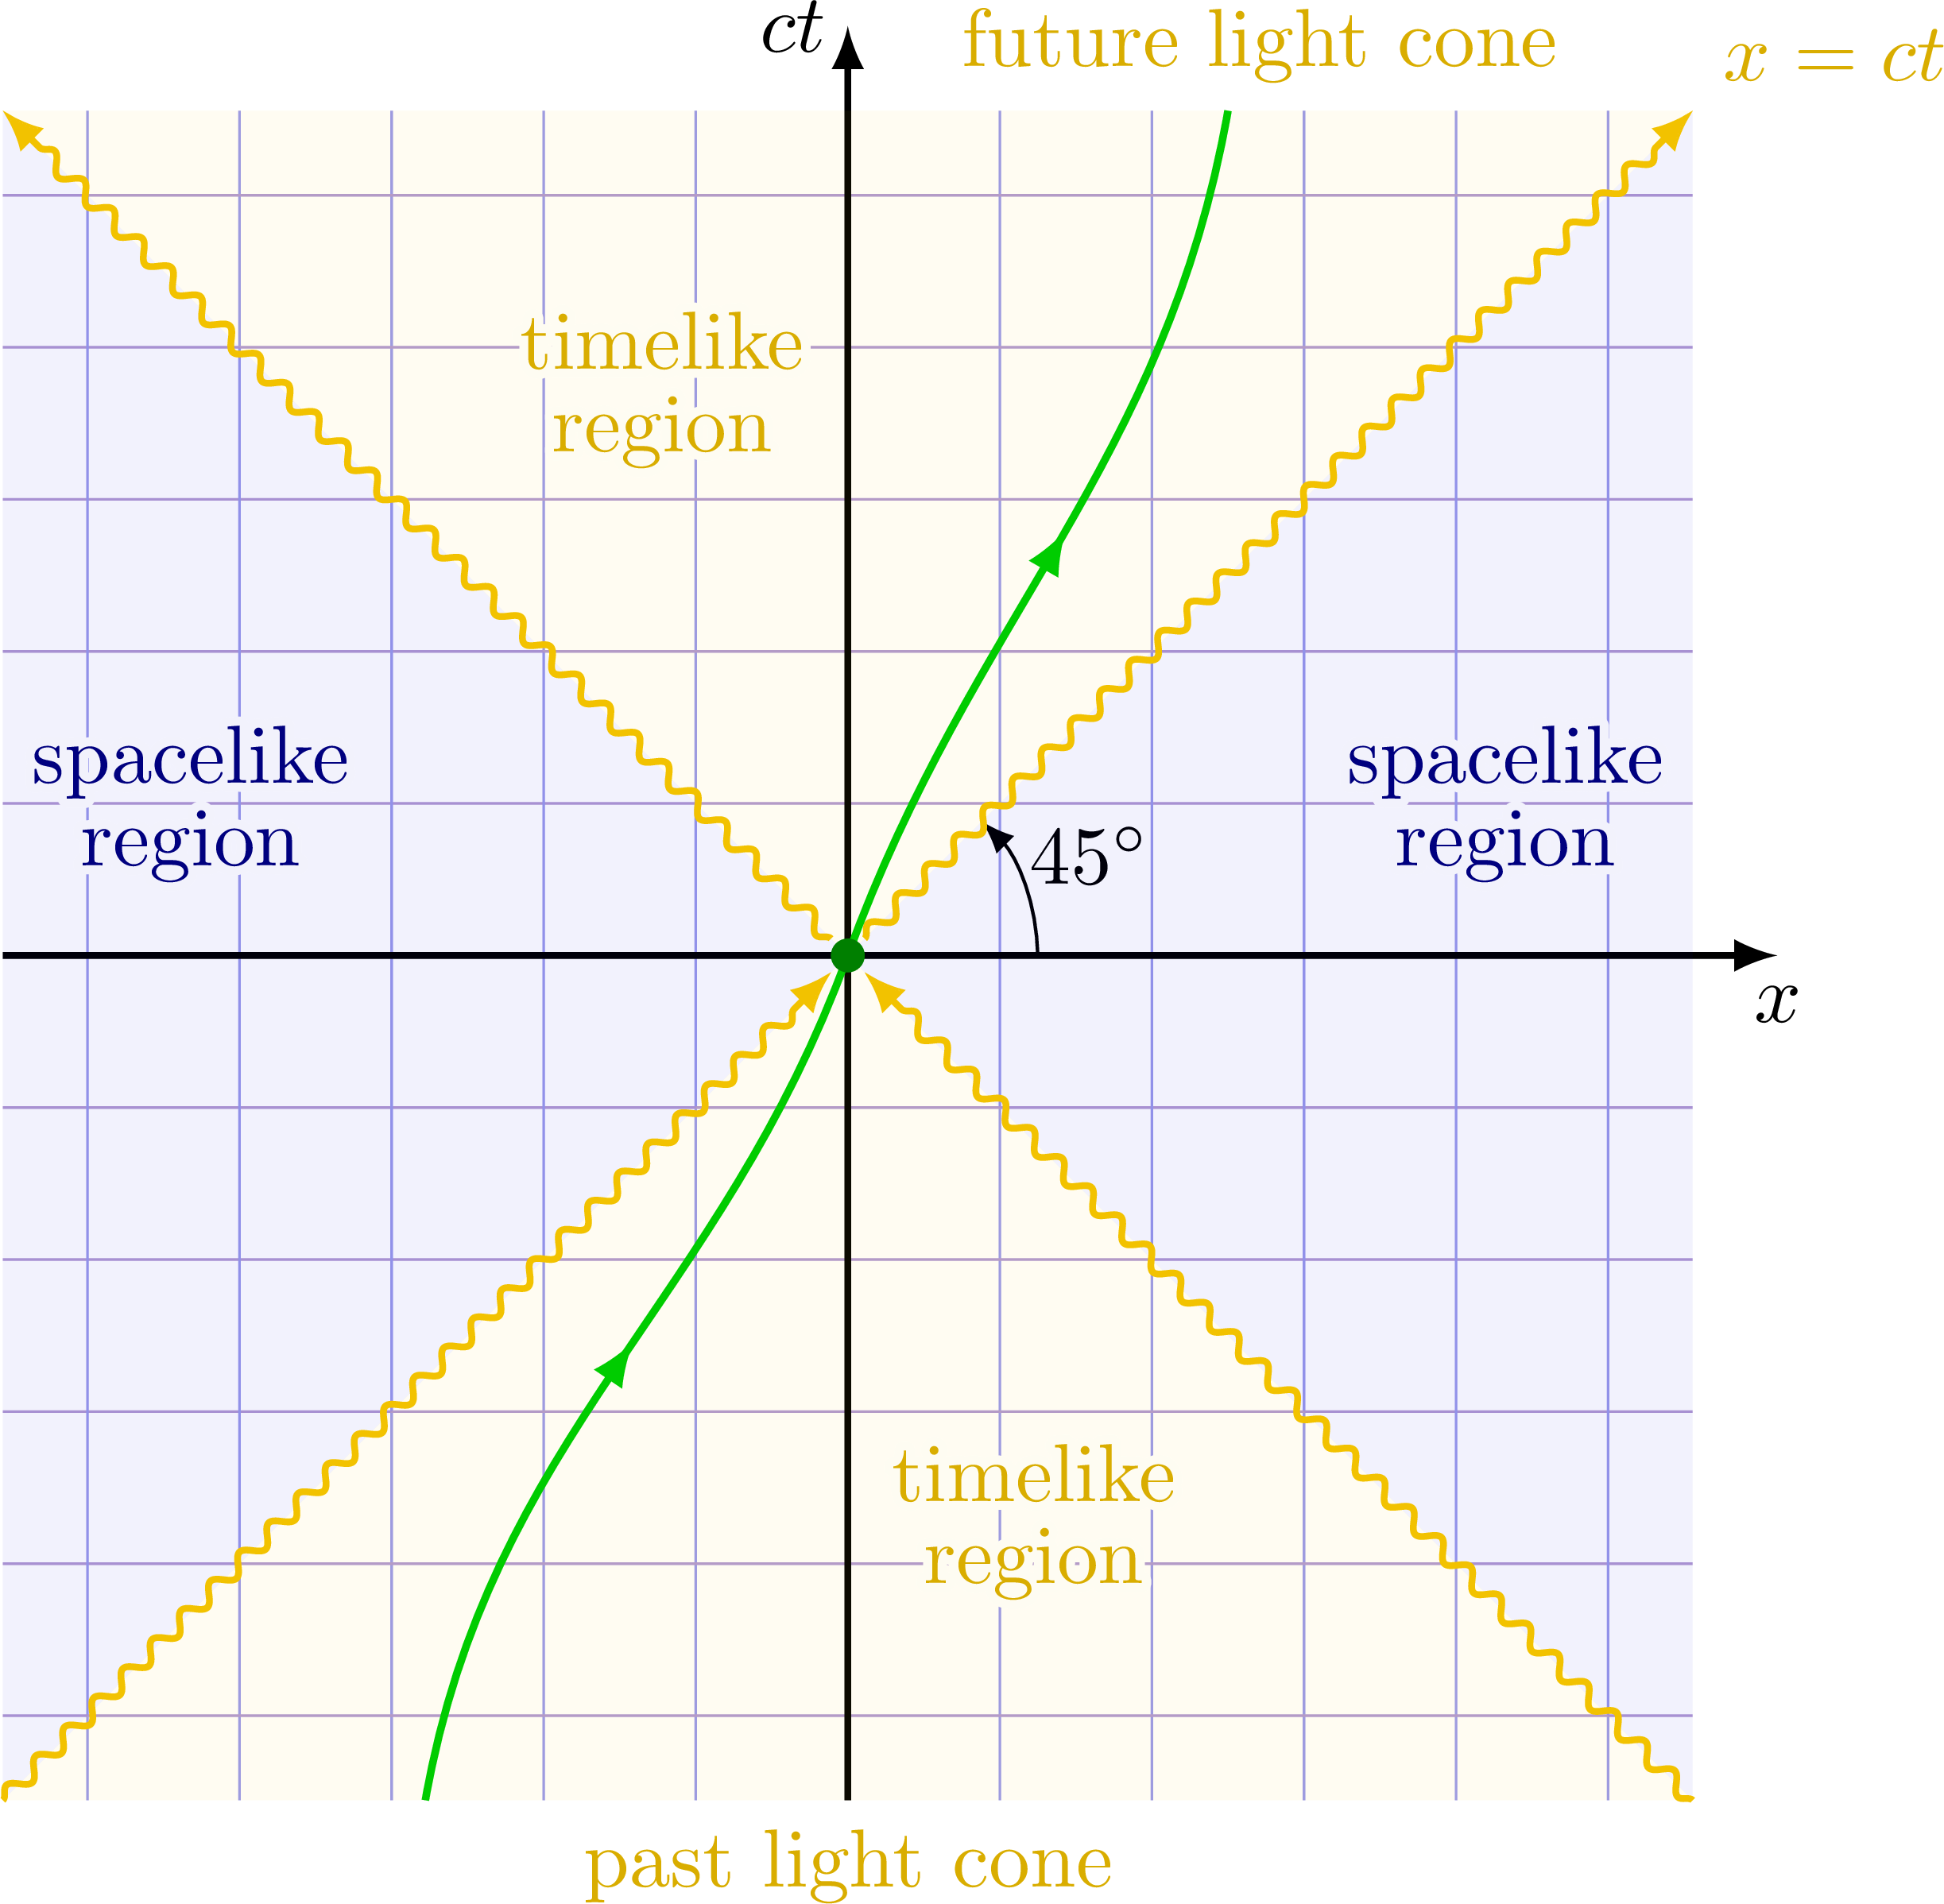
\includegraphics[width=0.85\linewidth]{./figures/tikz_3.png}
            \label{fig: tikz_3}
        \end{figure}
    \end{columns}
    \vfill
    \footnotetext{pgf – Create PostScript and PDF graphics in \TeX. \href{https://www.ctan.org/pkg/pgf}{\textcolor{hard_green}{https://www.ctan.org/pkg/pgf}}.}
\end{frame}


    % ---------------
% TIPS AND TRICKS
% ---------------

% Defining TOC's sections before content
\section{Tips \&\;tricks}

\begin{frame}
    \vfill
    \begin{center}
        \large
        Tips \&\;tricks
    \end{center}
    \vfill
\end{frame}

\begin{frame}
    \frametitle{ Tips \&\;tricks}
    \underline{Modules}:
    \begin{itemize}
        \item[$\diamond$] \textcolor{hard_green}{\textit{beamer}}\footnotemark permet de fabriquer des présentations/poster
        \footnotetext{beamer – A \LaTeX\;class for producing presentations and slides. \href{https://www.ctan.org/pkg/beamer}{\textcolor{hard_green}{https://www.ctan.org/pkg/beamer}}.}
        \item[$\diamond$] \textcolor{hard_green}{\textit{todonotes}}\footnotemark pour mettre des notes dans la marge
        \footnotetext{todonotes – Marking things to do in a \LaTeX document. \href{https://www.ctan.org/pkg/todonotes}{\textcolor{hard_green}{https://www.ctan.org/pkg/todonotes}}.}
    \end{itemize}
    \vfill
    \pause
    \underline{Sites internets}:
    \begin{itemize}
        \item[$\diamond$] \href{https://detexify.kirelabs.org/classify.html}{\textcolor{sweet_refs}{Detexify}} pour trouver des symboles \LaTeX\;grâce à un croquis en temps réel
        \item[$\diamond$] \href{https://mathpix.com/}{\textcolor{sweet_refs}{Mathpix}} pour obtenir le code \LaTeX\;d'une capture d'écran ou d'un fichier .pdf
    \end{itemize}
    \vfill
    \pause
    \underline{Templates}:
    \begin{itemize}
        \item[$\diamond$] \href{https://github.com/LJerome94/TeX-JAM/tree/main}{\textcolor{sweet_refs}{LJerome94/TeX-JAM}}
        \item[$\diamond$] \href{https://github.com/BCarnaval/UniTeX}{\textcolor{sweet_refs}{BCarnaval/UniTeX}}
        \item[$\diamond$] \href{https://www.overleaf.com/latex/templates}{\textcolor{sweet_refs}{Overleaf}}
    \end{itemize}
\end{frame}


\end{document}
